\documentclass[../main]{subfiles}

% Chapter 1: an introduction-type chapter. It shows the chapter opening
% (epigraph + chapter abstract), the full sectioning hierarchy, titled
% \paragraph and \subparagraph subtopics, the \subsectionclose and
% \sectionclose markers, footnotes, equations, a single-panel figure,
% citations and the acronym rules. Each sentence sits on its own source line.

\begin{document}
\chapter{Introduction}
\label{ch:ch1}
% Epigraph: chquote, wrapped in otherlanguage when it is not in English.
\begin{otherlanguage}{spanish}
\begin{chquote}
Esta es una cita de ejemplo,  \\
escrita en otro idioma.  \\
\bigskip
-- Autor, \textit{Obra} (I)
\end{chquote}
\end{otherlanguage}

% Chapter abstract: two or three italic sentences at the foot of the opening
% page. It brings its own \vfill. Headings and the chabstract do not count
% as acronym occurrences, so spell terms out here.
\begin{chabstract}
This is the chapter abstract, set in italics at the foot of the opening page.
It summarizes in two or three sentences what the chapter does, here the background of the thesis.
\end{chabstract}

% The body text starts overleaf.
\clearpage

The chapter opens with an untitled lead-in that states its scope.
The first occurrence of an acronym in the body text of a chapter is expanded with \verb|\acrfull|, as in \acrfull{bdg}, and every later one is short, \acrshort{bdg}.
Plurals use \verb|\acrfullpl| and \verb|\acrshortpl|, as in \acrfullpl{abs} and later \acrshortpl{abs}.
Every acronym links to the List of Abbreviations.
\lipsum[1][1-4]
In Section~\ref{sec:background} we review the background, and in Section~\ref{sec:thisthesis} we outline the rest of the thesis.

% ── Section ──────────────────────────────────────────────────
% Section and subsection titles spell acronyms out with \acrlong.
\section{Background on the \acrlong{dos}}
\label{sec:background}
A section starts with a short untitled lead-in before its first subsection.
It cites the literature with a non-breaking space before the bracket~\cite{Brown:PRB19}, and groups several references in a single \verb|\cite|, ordered oldest first~\cite{Muller:96, Brown:PRB19, Smith:PRL20}.
The \acrfull{dos} enters here for the first time in the body text.
\lipsum[2][1-5]

% ── Subsection with untitled paragraphs ─────────────────────
\subsection{Equations and figures}
\label{sec:equations}
A subsection with fewer than three subtopics keeps its paragraphs untitled.
Equations are part of the sentence that introduces them, which reads
\begin{equation}
    \label{eq:example}
    H = \frac{p^2}{2m^*} - \mu + \alpha\left(\sigma_x p_y - \sigma_y p_x\right)\tau_z + \Delta\tau_x,
\end{equation}
where every symbol is defined right after the equation.
A reference to it reads Eq.~\eqref{eq:example}, with a non-breaking space.
Multi-line expressions use \verb|split| inside \verb|equation|,
\begin{equation}
    \label{eq:split}
    \begin{split}
        E_\pm(k) &= \pm\sqrt{\xi_k^2 + \Delta^2}, \\
        \xi_k &= \frac{k^2}{2m^*} - \mu,
    \end{split}
\end{equation}
or \verb|align| when each line needs its own number,
\begin{align}
    \label{eq:align1}
    G &= \frac{2e^2}{h}\sum_n \transm_n, \\
    \label{eq:align2}
    I(\phi) &= \frac{e\Delta}{2\hbar}\sum_n \frac{\transm_n\sin\phi}{\sqrt{1 - \transm_n\sin^2(\phi/2)}}.
\end{align}
Quantum states use the \verb|physics| package, $\ket{\psi}$, $\braket{\psi}{\phi}$ and $\mel{\psi}{H}{\phi}$.
\lipsum[3][1-4]

% Figure placement: after the heading of the first (sub)section that
% references it, never before; preferably after the first \ref in the text.
Figure~\ref{fig:mock_single} shows the \acrshort{dos} of two mock models.
Figures are generated in external code repositories and only the rendered PDF is copied into \verb|ch1/figures/|.

\begin{figure}[hbtp]
    \centering
    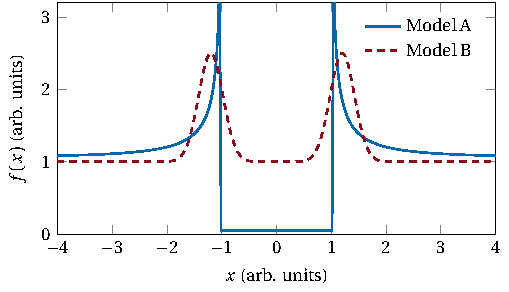
\includegraphics{figures/mock_single.pdf}
    % The optional argument is the short title in the List of Figures.
    % The caption opens with a bold one-line summary; a caption is read out
    % of order, so it expands its first acronym again with \acrfull.
    \caption[A single-panel mock-up figure]{\textbf{A single-panel mock-up figure of the \acrfull{dos}.}
    Each caption sentence sits on its own source line.
    The solid curve corresponds to model A and the dashed curve to model B, in arbitrary units.
    Later caption occurrences of the acronym are short, as in \acrshort{dos}.
    }
    \label{fig:mock_single}
\end{figure}

\lipsum[4][1-5]
A footnote goes right after the word or punctuation it qualifies\footnote{Inside a footnote, sentences are separated by single newlines only.
A blank line inside a macro argument breaks compilation.}.

% ── Subsection with titled \paragraph subtopics ─────────────
% Title \paragraphs only when the subsection has three or more subtopics of
% real length. \paragraph titles use \acrshort.
\subsection{Subtopics of a subsection}
\label{sec:subtopics}
An untitled lead-in can open a subsection whose subtopics are titled.
\lipsum[5][1-3]

\paragraph{First subtopic on the \acrshort{dos}}
\lipsum[6][1-6]

\paragraph{Second subtopic}
\lipsum[7][1-6]

\paragraph{Third subtopic, with \texttt{\textbackslash subparagraph}s}
A \verb|\paragraph| can be split further into \verb|\subparagraph|s.

\subparagraph{First case}
\lipsum[8][1-4]

\subparagraph{Second case}
\lipsum[9][1-4]

\subparagraph{Third case}
\lipsum[10][1-4]

% \subsectionclose (one asterisk) marks a synthesis of the whole subsection,
% across its \paragraphs, instead of giving it a heading of its own.
\subsectionclose
This closing paragraph summarizes the three subtopics of the subsection and bridges to the next one.
\lipsum[11][1-3]

% ── Subsection with subsubsections ──────────────────────────
\subsection{A subsection with subsubsections}
\label{sec:subsubsections}
\lipsum[12][1-3]

\subsubsection{First subsubsection}
\lipsum[13][1-5]

% A (sub)subsection adapted from a published paper gets a footnote on its
% title, inside the optional short title so the footnote stays out of the
% table of contents and the running head.
\subsubsection[Second subsubsection, adapted from a paper]{Second subsubsection, adapted from a paper\footnote{Section~\ref{sec:adapted_subsection} is adapted from Ref.~\cite{Doe:a26}.}}
\label{sec:adapted_subsection}
\lipsum[14][1-5]

% \sectionclose (two asterisks) marks a synthesis of the whole section,
% across its subsections.
\sectionclose
This closing paragraph summarizes the whole section.
\lipsum[15][1-3]

% ── Last section: outline of the thesis ─────────────────────
\section{This thesis}
\label{sec:thisthesis}
The last section of the introduction outlines the chapters that follow.
Chapter~\ref{ch:ch2} presents the main results, and Chapter~\ref{ch:ch3} draws the conclusions.
Appendix~\ref{app:example} collects technical details.
An acronym used only once in the body text of a chapter is spelled out with \verb|\acrlong|, as the \acrlong{twodeg} here.
\lipsum[16]

% Standalone build of this chapter: print its own bibliography.
\ifSubfilesClassLoaded{%
\newrefcontext[labelprefix=]
\printbibliography
}{}
\end{document}
